\chapter{Malpasset dambreak (malpasset)}

\section{Purpose}

This test illustrates that \telemac{3D} is able to simulate a real dam break flow on an initially dry domain. It also shows the propagation of the wave front and the evolution in time of the water surface and velocities in the valley downstream. It was used as a test case in the program ESPRIT for the european project PCECOWATER (Parallel Computing of Environment COastal and lake shallow WATER dynamics).

\section{Description}

This case is the simulation of the propagation of the wave following the break of the Malpasset dam
(South-East of France). This accident occurred in December 1959.
The model represents the reservoir upstream from the dam and the valley and flood plain downstream.
The entire valley is approximately 18~km long and between 200~m (valley) and 7~km wide (flood plain).
The complete study is described in details in \cite{Hervouet2007}.
The simulation is performed using 2 or 6 vertical planes (cases MURD P2 and MURD P6)
using the treatment of negative depths introduced since \telemac{3D} 7.0.
The historical simulation using 2 vertical planes and the method of characteristics (named CHAR P2)
has been kept. Nevertheless, the recommended advection scheme for velocities for such applications
is now the N-type MURD scheme (14). A simulation using 2 vertical planes with a large mesh
(FINE P2) is also performed, but only in parallel to save CPU time.
The characteristics of the case are the following:
\begin{itemize}
  \itemsep0em
\item Observed mean wave velocity $U_0$ = 27~km.h$^{-1}$ = 7.5~m.s$^{-1}$,
\item Initial water depth upstream of the dam $H_0$ = 55~m,
\item Total duration of the event $T$ = 4,000~s,
\item Valley length $L$ = 18~km,
\item Maximum valley width $l_M$ = 7~km,
\item Reynolds Number \textbf{$R_e = \dfrac{U_0 \times H_0}{\nu} =  4.12 \times 10^8$} where $\nu$ is the kinematic viscosity of water,
\item Froude Number \textbf{$F_r = \dfrac{U_0}{\sqrt{g \times H_0}} = 0.32$} where $g$ is the gravity acceleration.
\end{itemize}.

\subsection{Geometry and Mesh}
The size of the model is approximately  17~km $\times$ 9~km. The mesh is refined in the river valley (downstream from the dam) and on the banks.
Two 2D triangular meshes are tested: \\
\textbf{Regular mesh (Figure \ref{fig:malpasset:Mesh} - a):}
\begin{itemize}
\itemsep0em
\item 26,000 triangular elements,
\item 13,541 nodes,
\item Maximum size range is from 17 to 313~m.
\end{itemize}
\textbf{Fine mesh (Figure \ref{fig:malpasset:Mesh} - b):}
\begin{itemize}
\itemsep0em
\item 104,000 triangular elements,
\item 53,081 nodes,
\item Maximum size range is from 8.5 to 156.5~m.
\end{itemize}
\begin{figure}[H]
  \centering
  \textbf{a - Regular mesh}\par\medskip
  \includegraphicsmaybe{[width=0.7\textwidth]}{../img/Mesh_small.png} \\
  \textbf{b - Fine mesh}\par\medskip
  \includegraphicsmaybe{[width=0.7\textwidth]}{../img/Mesh_large.png}
  \caption{Malpasset case meshes.}\label{fig:malpasset:Mesh}
\end{figure}
In this 2D mesh, the dam is modelled by a straight line between the points of
coordinates (4,701.18 m ; 4,143.10 m) and (4,655.50 m ; 4,392.10 m).
Its location is shown in Figure \ref{fig:malpasset:mesh_dam}.
For the construction of the 3D mesh, two discretizations with 2 or 6 layers regularly spaced on the
vertical are tested.
\begin{figure}[H] %Example
  \centering
  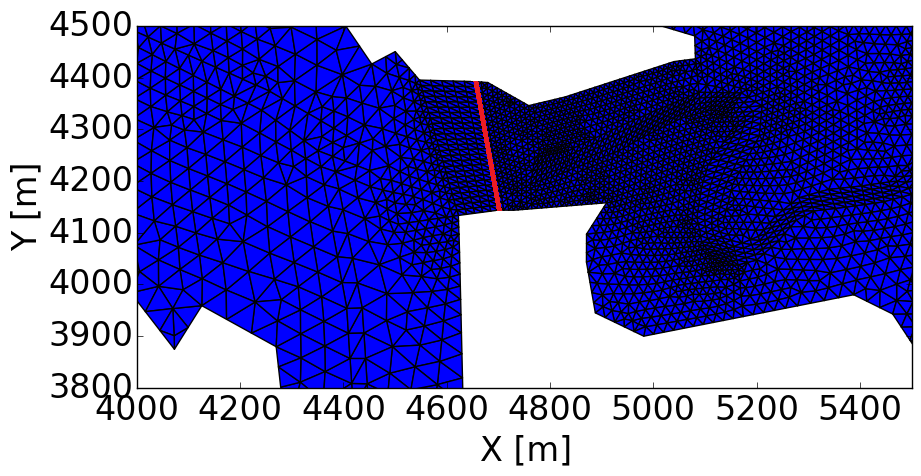
\includegraphics[width=0.7\textwidth]{img/Mesh_small_dam.png}
  \caption{Dam location on the Malpasset case.}\label{fig:malpasset:mesh_dam}
\end{figure}

\subsection{Bathymetry}
Old maps have been used to deduce the topography of the domain (Figure \ref{fig:malpasset:bathy}).
In fact, the topography after the accident could not be used because of the dramatic changes
that occured. Therefore, the IGN map of Saint-Tropez, Number 3, of year 1931, was used.

\begin{figure}[H]
  \centering
  \includegraphicsmaybe{[width=\textwidth]}{../img/bathymetry.png}
  \caption{Bottom levels in the domain of the Malpasset case and reference points.}
  \label{fig:malpasset:bathy}
\end{figure}

\subsection{Numerical parameters}

\subsection{Initial conditions}
At the beginning of the simulation, the dam is assumed undamaged and the reservoir is full. There is no water in the downstream valley, and no velocity in all the domain.
\subsection{Boundary conditions}
The boundaries are solid everywhere and the channel banks considered as solid walls. There is no friction on the solid walls. The bottom is considered as a solid boundary with roughness. The Strickler formula with friction coefficient = 30~m$^{1/3}$/s is used.

\subsection{Cases}
For this test case, four different simulations are run. The following characteristics are common to all cases:\\
\begin{itemize}
\itemsep0em
\item Type of computation: Non-hydrostatic,
\item Duration: 4,000~s.
\end{itemize}

The simulation parameters specific to each case are summed up in Table \ref{tab:malpasset:cases}.
\begin{table}[H]
  \resizebox{\textwidth}{!}{
    \begin{tabular}{|c|c|c|c|c|c|c|}
      \hline Case & Name & Mesh & Number of vertical planes & Advection scheme for velocities & Time step \\
      \hline 1 & MURD P2 & Regular & 2 & N-type MURD & 4.0~s \\
      \hline 2 & CHAR P2 & Regular & 2 & Characteristics & 4.0~s \\
      \hline 3 & MURD P6 & Regular & 6 &  N-type MURD  & 4.0~s \\
      \hline 4 & FINE P2 & Fine & 2 & N-type MURD & 1.0~s \\
      \hline
    \end{tabular}
  }
  \caption{List of the simulation parameters used for the four cases tested in the Malpasset example.}
  \label{tab:malpasset:cases}
\end{table}

\subsection{Physical parameters}
In the simulations, the Coriolis force and the wind effect are not taken into account. Besides, the viscosity is set as constant and equal to 1~m$^2$/s on horizontal directions.

\section{Results}

\subsection{First observations}
Figure \ref{fig:malpasset:WD_MURD_P2} illustrates the progression of the flood wave after the dam
break (simulation MURD P2 with scheme N-type MURD using the treatment of negative depths that
smoothes the results on tidal flats). %The propagation of the wave front is very fast.
%The water depths rapidly increase in the valley downstream from the dam location.
%The wave spreads in the plain when arriving to the sea.
%Instabilites appear at the downstream boundary.

\begin{figure}[H]
  \centering
  \textbf{t = 0.0~s}\par\medskip
  \includegraphicsmaybe{[width=0.8\textwidth]}{../img/WD0_MURD_P2.png}\\
  \textbf{t = 200.0~s}\par\medskip
  \includegraphicsmaybe{[width=0.8\textwidth]}{../img/WD200_MURD_P2.png}\\
  \textbf{t = 600.0~s}\par\medskip
  \includegraphicsmaybe{[width=0.8\textwidth]}{../img/WD600_MURD_P2.png}\\
  \textbf{t = 2400.0~s}\par\medskip
  \includegraphicsmaybe{[width=0.8\textwidth]}{../img/WD2400_MURD_P2.png}
  \caption{Evolution of the water depth in time for Case MURD P2 on the Malpasset example.}\label{fig:malpasset:WD_MURD_P2}
\end{figure}
Figure \ref{fig:malpasset:WD_all} shows the water depth at time 400~s obtained with 2
planes (MURD P2), 6 planes (MURD P6) and the treatment of negative depths,
2 planes using the method of characteristics (CHAR P2) and 2 planes using the fine mesh
(FINE P2) calculations. The results are similar for simulations using the MURD scheme with 2 and
6 planes. The characteristics scheme gives comparable results.
The wave seems to propagate faster with the fine mesh.
Figures \ref{fig:malpasset:velocityFieldMURD} show the velocity field after 100~s in the vicinity of the dam for 3 XY planes of case MURD P6.
\begin{figure}[H]
  \centering
  \textbf{POS P2}\par\medskip
  \includegraphicsmaybe{[width=0.8\textwidth]}{../img/WD400_MURD_P2.png}\\
  \textbf{POS P6}\par\medskip
  \includegraphicsmaybe{[width=0.8\textwidth]}{../img/WD400_MURD_P6.png}\\
  \textbf{CHAR P2}\par\medskip
  \includegraphicsmaybe{[width=0.8\textwidth]}{../img/WD400_CHAR_P2.png}\\
  \textbf{Large P2}\par\medskip
  \includegraphicsmaybe{[width=0.8\textwidth]}{../img/WD400_FINE_P2.png}
  \caption{Water depth at 400~s for the studied cases on the Malpasset example.}\label{fig:malpasset:WD_all}
\end{figure}



\begin{figure}[H]
  \centering
  \textbf{Plane 1 (Bottom)}\par\medskip
  \includegraphicsmaybe{[width=0.6\textwidth]}{../img/Velocity100_MURD_P6_plane1.png}\\
  \textbf{Plane 3}\par\medskip
  \includegraphicsmaybe{[width=0.6\textwidth]}{../img/Velocity100_MURD_P6_plane3.png}\\
  \textbf{Plane 6 (Free Surface)}\par\medskip
  \includegraphicsmaybe{[width=0.6\textwidth]}{../img/Velocity100_MURD_P6_plane6.png}
  \caption{Velocity field for case POS P6 after 100 s on the Malpasset example.}\label{fig:malpasset:velocityFieldMURD}
\end{figure}

The effect of the bend is noticeable even in this early stage of the simulation for all the planes.
In fact, a recirculation can be observed on the right bank in the three figures. \\

Velocity values are compared in Figure \ref{fig:malpasset:velocityMap} for the same three planes. The free surface velocity values are slightly higher than near the bottom.

\begin{figure}[H]
  \centering
  \hspace{-1.cm}\textbf{Plane 1 (Bottom)}\par\medskip
  \includegraphicsmaybe{[width=0.7\textwidth]}{../img/VelocityMap100_MURD_P6_plane1.png}\\
  \hspace{-1.cm}\textbf{Plane 3}\par\medskip
  \includegraphicsmaybe{[width=0.7\textwidth]}{../img/VelocityMap100_MURD_P6_plane3.png}\\
  \hspace{-1.cm}\textbf{Plane 6 (Free Surface)}\par\medskip
  \includegraphicsmaybe{[width=0.7\textwidth]}{../img/VelocityMap100_MURD_P6_plane6.png}
  \caption{Velocity values for case POS P6 after 100 s on the Malpasset example.}\label{fig:malpasset:velocityMap}
\end{figure}

\subsection{Comparison of schemes}
\subsubsection*{Performance}
Performance tests are conducted on the cases. The studied variable here is the water depth.\\

%First, a none-regression test is done comparing the results (water depth) of the schemes with references (older results using older version of TELEMAC2D). The error norms (Table \ref{tab:malpasset:NonReg}) can be compared to the machine precision ($2.2204460492 * 10^{-16}$).
%
%\begin{table}[H]
%\centering
%\begin{tabular}{|l|}
%  \hline \\
%  \hline  Pos P2 \\
%  Charac P2 \\
%  Pos P6 \\
%  Large \\
%  \hline
%\end{tabular}%
%\begin{tabular}{|c|c|c|}
%  \hline $||\epsilon||_{L^1}$ & $||\epsilon||_{L^2}$ & $||\epsilon||_{L^{\infty}}$ \\
%  \hline
%  \InputIfFileExists{../NonReg.txt}{}{}\\
%  \hline
%\end{tabular}
%  \caption{None-regression test of water depth values.}
%  \label{tab:malpasset:NonReg}
%\end{table}

Times of simulation for each  of these cases with sequential and parallel runs (using 4 processors) are shown in Table \ref{tab:malpasset:SeqParTimes} \footnote{Keep in mind that these times are specific to the validation run and the type of the processors that were used for this purpose.}.
Remember that the computation with the fine mesh is only run in parallel to save CPU time and no result is shown in sequential for it.

\begin{table}[H]
  %\resizebox{\textwidth}{!}
  \caption{Time of simulation for different cases of the Malpasset example.}
  \label{tab:malpasset:SeqParTimes}
\end{table}

With the regular 2D mesh and 2 planes on the vertical, the fastest scheme is the characteristics. Nevertheless, the MURD scheme simulation time is only few seconds longer.

Obviously, increasing the number of planes or the number of 2D elements makes the simulation much longer. Further more, parallel runs using 4 processors considerably decrease simulation times.

Sequential and parallel simulations results are compared for each case in Table \ref{tab:malpasset:SeqPar}. That allows to quantify the loss of information that goes along with the partitioning of the mesh.
\begin{table}[H]
  \centering
  \begin{tabular}{|l|}
    \hline \\
    \hline  MURD P2 \\
    CHAR P2 \\
    MURD P6 \\
%    FINE P2 \\ % no more sequential run for the fine mesh
    \hline
  \end{tabular}
  \begin{tabular}{|c|c|c|}
    \hline $||\epsilon||_{L^1}$ & $||\epsilon||_{L^2}$ & $||\epsilon||_{L^{\infty}}$ \\
    \hline
    \InputIfFileExists{../SeqPar.txt}{}{}\\
    \hline
  \end{tabular}
  \caption{Sequential VS Parallel - Errors on water depth values on the Malpasset case.}
    \label{tab:malpasset:SeqPar}
\end{table}

\subsubsection*{Accuracy}
In order to evaluate the precision of the tested schemes, the results are compared to data obtained from:
\begin{itemize}
\itemsep0em
\item  A physical model (see \cite{Hervouet2007}) (Non-distorted, 1/400 scale) that was built in LNHE (EDF) in 1964, from which measurements of the free surface were taken using gauges put in different locations,
\item Reality. In fact, three electric transformers (called A, B and C from upstream to downstream) were destroyed by the wave and the the times of electric shutdowns were precisely recorded.
\end{itemize}

The locations of these observation points are shown in Figure \ref{fig:malpasset:MeasurePoints}.
\begin{figure}[H]
  \centering
  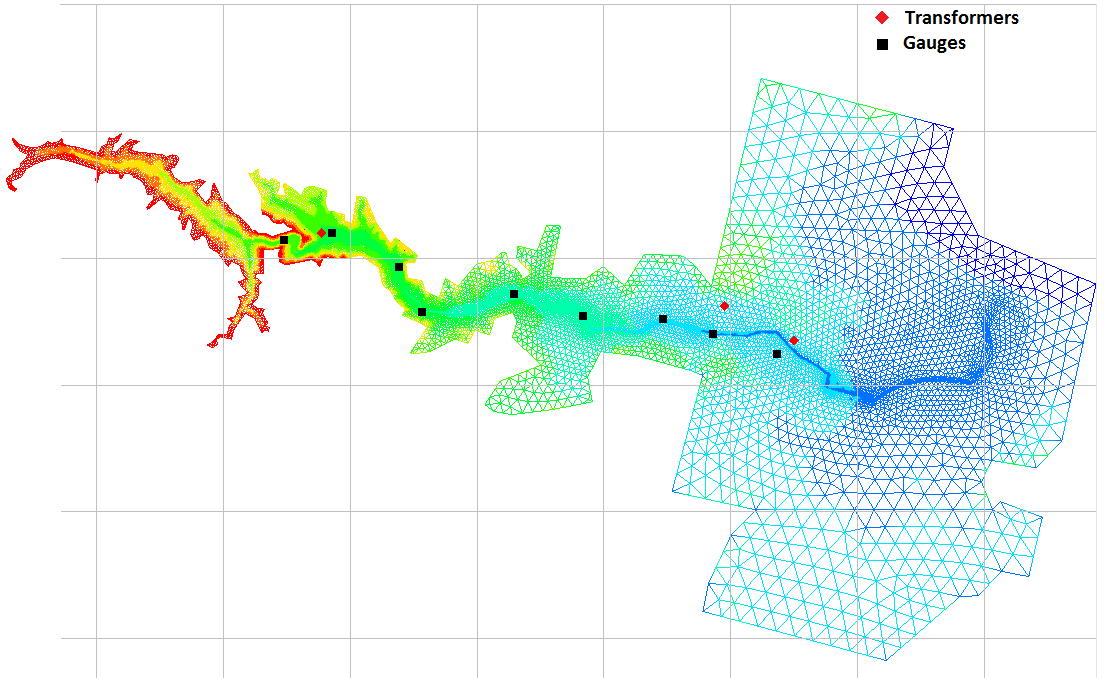
\includegraphics[width=1.0\textwidth]{img/MeasurePoints.png}
  \caption{location of gauges (physical model) and transformers (field) represented on the mesh of the Malpasset case.}\label{fig:malpasset:MeasurePoints}
\end{figure}

The measured data used in this document are the following:
\begin{itemize}
\itemsep0em
\item Recorded time from A (5,550~m ; 4,400~m) to B (11,900~m ; 3,250~m) : 1,140.0~s,
\item Recorded time from A to C (13,000~m ; 2,700~m): 1,320.0~s,
\item Maximum free surface elevations obtained from gauges. The values are converted to water depths (by deducing the bathymetry values) and summed up in Table \ref{tab:malpasset:MaxMeasures}.
\end{itemize}

\begin{table}[H]
  \centering
  \begin{tabular}{|c|c|c|c|c|}
    \hline Point Name & $x$-coordinate & $y$-coordinate & Distance to dam & Measured Max water depth \\
    \hline P6 & 4,947 & 4,289 & 336 & 40.3\\
    P7 & 5,717 & 4,407 & 1,320 & 14.6\\
    P8 & 6,775 & 3,869 & 2,160 & 24.0\\
    P9 & 7,128 & 3,162 & 3,420 & 12.8\\
    P10 & 8,585 & 3,443 & 4,840 & 11.8 \\
    P11 & 9,674 & 3,085 & 6,000 & 8.3\\
    P12 & 10,939 & 3,044 & 7,220 & 10.1\\
    P13 & 11,724 & 2,810 & 7,980 & 6.8 \\
    P14 & 12,723 & 2,485 & 8,960 & 5.4\\
    \hline
  \end{tabular}
  \caption{Maximum values of water depth on measurement points of the Malpasset case (m).}
  \label{tab:malpasset:MaxMeasures}
\end{table}

These data are used to calculate the relative gap percentage between the physical model results and numerical model results. This error percentage is calculated as a $L^{1}$-type relative error given by $100 \times \dfrac{H_{telemac3d} - H_{gauge}}{H_{gauge}}$. The maximum values of water depth are extracted for each gauge for all the schemes and summed up in Table \ref{tab:malpasset:MaxTab}. Negative values of error percentage are colored in red and correspond to a numerical estimation lower than the observed one.
\begin{table}[H]
  \resizebox{\textwidth}{!}{
    \centering
    \begin{tabular}{|l}
      \hline Point \\
      \hline P6 \\
      P7 \\
      P8 \\
      P9 \\
      P10 \\
      P11 \\
      P12 \\
      P13 \\
      P14 \\
      \hline
    \end{tabular}
    \begin{tabular}{|c|c|c|c|}
      \hline  MURD P2 & CHAR P2 & MURD P6 & FINE P2\\
      \hline
      \InputIfFileExists{../img/MaxLevels_schemes.txt}{}{} \\
      \hline
  \end{tabular}}
  \caption{Maximum values of water depth on measurement points for different schemes on the Malpasset case - relative errors.}
      \label{tab:malpasset:MaxTab}
\end{table}

First deduction is that the number of planes does not seem to influence the results much (comparison between MURD P2 and MURD P6). The fine mesh improves the results for points 6 to 10, but the error percentages rise for points 11 to 14. \\

In general, for all the schemes, some points (eg. P14) seem to result with very high discrepancies in comparison with observed results. The following interpretation can be found in reference \cite{Hervouet2007}. \\

\textit{
« The discrepancies on the free surface elevation at the nine gauges, between 1-D and 2-D solutions, and the physical model, remain large and are questionable. However, the results are good as soon as the wave reaches the floodplain, the difference at gauge 14 being 14 cm with a total depth of 5.4 m. It is clear from the sensitivity study done with TELEMAC-2D that the differences are not entirely due to an inaccurate solution of the Shallow water equations. As a matter of fact, numerical and physical parameters have little influence on the maximum free surface elevation, but not in a range that would allow a possible perfect match. Several other factors could be responsible for the error such as:
\begin{itemize}
\itemsep0em
\item the physical model itself, because a 1/400 scale gives a 4~m difference for a 1cm error on measurements,
\item the Shallow Water equations are an approximation and their assumptions, such as the hydrostatics pressure, cannot be fully verified in this case - a test with Boussinesq or Serre equations would be of the utmost interest to clarify this point,
\item the dam failure scenario, which was probably not absolutely instantaneous,
\item the debris flow and sediment transport, which was not taken into account in this study»
\end{itemize}
}

Next, the propagation time of the wave recorded in \telemac{3D} is compared to
reality in Table \ref{tab:malpasset:waveTimes}.
Negative values of error percentage are colored in red and correspond to a
numerical estimation lower than the observed one.
\begin{table}[H]
  \resizebox{\textwidth}{!}{
    \centering
    \begin{tabular}{|l}
      \hline  Distance \\
      \hline A to B \\
      A to C \\
      \hline
    \end{tabular}
    \begin{tabular}{|c|c|c|c|}
      \hline  MURD P2 & CHAR P2 & MURD P6 & FINE P2\\
      \hline
      \InputIfFileExists{../img/waveTimes_schemes.txt}{}{} \\
      \hline
  \end{tabular}}
  \caption{Propagation time of the wave for different schemes on the Malpasset case - relative error.}
  \label{tab:malpasset:waveTimes}
\end{table}

The errors here have the same magnitude for the first three cases. The use of 6 planes does not improve the results. Nevertheless, the finer mesh gives better estimation of the A-B transit time.


\subsubsection*{Comparison on profiles}
Here, the schemes are compared on profiles upstream (Figure \ref{fig:malpasset:upstreamProfile}) and downstream (Figure \ref{fig:malpasset:downstreamProfile}) of the dam. The locations of these profiles are the following:
\begin{itemize}
\itemsep0em
\item Upstream of the dam: (4,634.0 ; 4,132.84) (4,589.81 ; 4,393.22),
\item Downstream of the dam: (4,884.95 ; 4,161.82) (4,846.39 ; 4,362.44).
\end{itemize}

\begin{figure}[H]
  \centering
  \includegraphicsmaybe{[width=0.6\textwidth]}{../img/WaterDepth_Dam_amont.png}
  \caption{Profiles of water depth upstream of the dam at last iteration of the Malpasset case.}\label{fig:malpasset:upstreamProfile}
\end{figure}
These figures show the following:
\begin{itemize}
\itemsep0em
\item The number of planes does not seem to influence the water depth profile,
\item The refinement of the 2D mesh has considerable influence,
\item The characteristics scheme seems to overestimate the values of the water depth as compared to the MURD scheme.
\end{itemize}
\begin{figure}[H]
  \centering
  \includegraphicsmaybe{[width=0.6\textwidth]}{../img/WaterDepth_Dam_aval.png}
  \caption{Profiles of water depth downstream of the dam at last iteration of the Malpasset case.}\label{fig:malpasset:downstreamProfile}
\end{figure}

\subsubsection*{Positivity}
Further more, the positivity of the used schemes can be checked for all cases. In order to achieve this, the minimum value of the water depth during the whole simulation, and on all the points of the mesh, is transcribed in Table \ref{tab:malpasset:NegCheck}.

\begin{table}[H]
  \resizebox{\textwidth}{!}{
    \centering
    \begin{tabular}{|l}
      \hline Schemes \\
      \hline Minimum $H$ [m] \\
      \hline
    \end{tabular}
    \begin{tabular}{|c|c|c|c|}
      \hline   MURD P2 & CHAR P2 & MURD P6 & FINE P2\\
      \hline \InputIfFileExists{../hmins.txt}{}{}\\
      \hline
  \end{tabular}}
    \caption{Minimum value of water depth through the simulation for each case of the Malpasset example.}
  \label{tab:malpasset:NegCheck}
\end{table}

\subsubsection*{Mass conservation}
Mass conservation can be checked by calculating the volume in the domain during time (as the density is constant in time and space). Lost volume is calculated as $V_{initial} - V_{final}$.
\begin{table}[H]
  \resizebox{\textwidth}{!}{
    \centering
    \begin{tabular}{|l|c}
      \hline   & \\
      \hline \textbf{Sequential} & Lost volume [m$^3$] \\
      & Relative error \\
      \hline \textbf{Parallel} & Lost volume [m$^3$] \\
      & Relative error \\
      \hline
    \end{tabular}
    \begin{tabular}{|c|c|c|c|}
      \hline  MURD P2 & CHAR P2 & MURD P6 & FINE P2\\
      \hline
      \InputIfFileExists{../img/volErrors_schemes.txt}{}{} \\
      \hline
      \InputIfFileExists{../img/volErrors_schemes_Parallel.txt}{}{} \\
      \hline
  \end{tabular}}
  \caption{Volume loss and relative error for different schemes of the Malpasset case.}
  \label{tab:malpasset:volumeTimes}
\end{table}

Table \ref{tab:malpasset:volumeTimes} shows that the schemes are conservative. Mass conservation is equivalent between sequential and parallel runs. The evolution of volume through time for each of the schemes is shown in Figure \ref{fig:malpasset:VoLTime} and vizually confirms the previous conclusion.

\begin{figure}[H]
\centering
  \includegraphicsmaybe{[width=0.7\textwidth]}{../img/VolTime.png}
  \caption{Evolution of water volume through time for the tested schemes on the Malpasset case.}
\label{fig:malpasset:VoLTime}
\end{figure}

\section{Conclusion}

\telemac{3D} is capable of simulating the propagation of a dam break wave in a river valley initially dry. The recommended scheme here is the N-type MURD scheme, as it gives a good approximation with the observed data, specially for the wave speed. Further more, the simulation time with the MURD scheme is equivalent to that with the characteristics scheme.
Moreover, in this test case, a higher number of planes does not improve the results, but a refinement of the 2D mesh does.
Unfortunately, for the latter, simulation time increases considerably.
